% Created by tikzDevice version 0.6.2-92-0ad2792 on 2013-11-12 07:52:59
% !TEX encoding = UTF-8 Unicode
\documentclass[12pt, mainfont = Minion,     mainscale = 1.0, sansfont = Myriad,     sansscale = MatchLowercase, monofont = Consolas,   monoscale = MatchLowercase, mathfont = MinionMath, mathscale = 1.0]{mtikzfig}
\begin{document}

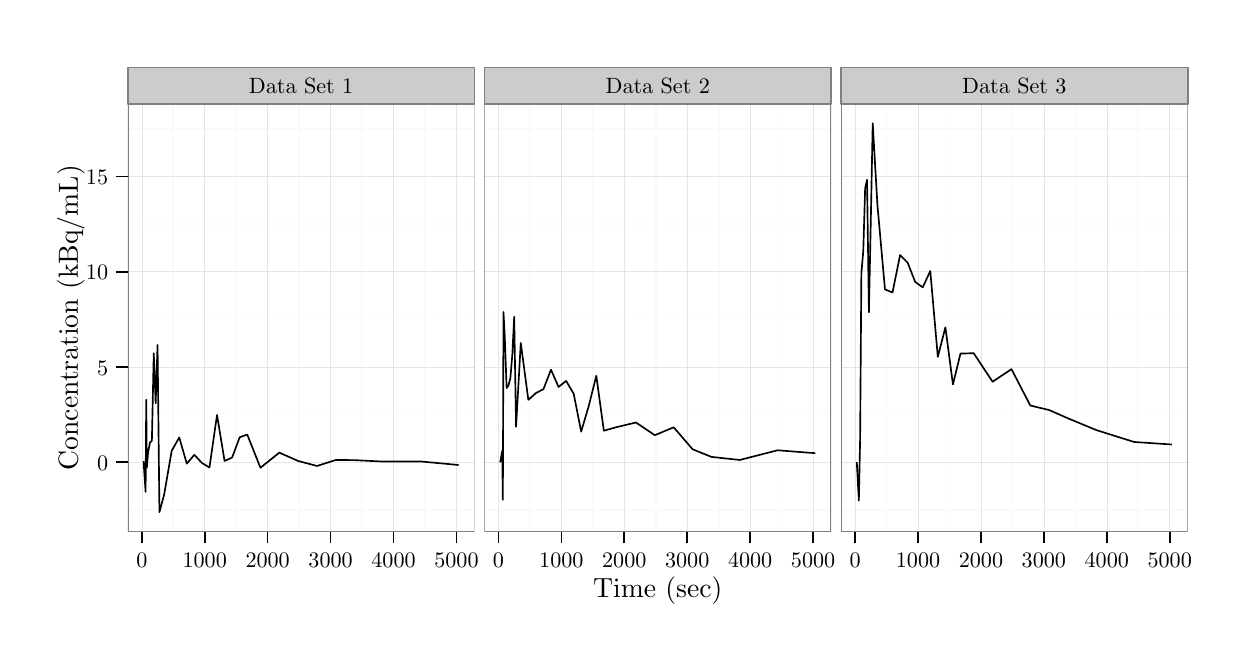
\begin{tikzpicture}[x=1pt,y=1pt]
\definecolor[named]{fillColor}{rgb}{1.00,1.00,1.00}
\path[use as bounding box,fill=fillColor,fill opacity=0.00] (0,0) rectangle (433.62,216.81);
\begin{scope}
\path[clip] (  0.00,  0.00) rectangle (433.62,216.81);
\definecolor[named]{drawColor}{rgb}{1.00,1.00,1.00}
\definecolor[named]{fillColor}{rgb}{1.00,1.00,1.00}

\path[draw=drawColor,line width= 0.6pt,line join=round,line cap=round,fill=fillColor] (  0.00,  0.00) rectangle (433.62,216.81);
\end{scope}
\begin{scope}
\path[clip] ( 36.18, 34.74) rectangle (161.43,189.27);
\definecolor[named]{fillColor}{rgb}{1.00,1.00,1.00}

\path[fill=fillColor] ( 36.18, 34.74) rectangle (161.43,189.27);
\definecolor[named]{drawColor}{rgb}{0.98,0.98,0.98}

\path[draw=drawColor,line width= 0.6pt,line join=round] ( 36.18, 42.58) --
	(161.43, 42.58);

\path[draw=drawColor,line width= 0.6pt,line join=round] ( 36.18, 76.99) --
	(161.43, 76.99);

\path[draw=drawColor,line width= 0.6pt,line join=round] ( 36.18,111.41) --
	(161.43,111.41);

\path[draw=drawColor,line width= 0.6pt,line join=round] ( 36.18,145.82) --
	(161.43,145.82);

\path[draw=drawColor,line width= 0.6pt,line join=round] ( 36.18,180.24) --
	(161.43,180.24);

\path[draw=drawColor,line width= 0.6pt,line join=round] ( 52.61, 34.74) --
	( 52.61,189.27);

\path[draw=drawColor,line width= 0.6pt,line join=round] ( 75.35, 34.74) --
	( 75.35,189.27);

\path[draw=drawColor,line width= 0.6pt,line join=round] ( 98.09, 34.74) --
	( 98.09,189.27);

\path[draw=drawColor,line width= 0.6pt,line join=round] (120.83, 34.74) --
	(120.83,189.27);

\path[draw=drawColor,line width= 0.6pt,line join=round] (143.57, 34.74) --
	(143.57,189.27);
\definecolor[named]{drawColor}{rgb}{0.90,0.90,0.90}

\path[draw=drawColor,line width= 0.2pt,line join=round] ( 36.18, 59.79) --
	(161.43, 59.79);

\path[draw=drawColor,line width= 0.2pt,line join=round] ( 36.18, 94.20) --
	(161.43, 94.20);

\path[draw=drawColor,line width= 0.2pt,line join=round] ( 36.18,128.61) --
	(161.43,128.61);

\path[draw=drawColor,line width= 0.2pt,line join=round] ( 36.18,163.03) --
	(161.43,163.03);

\path[draw=drawColor,line width= 0.2pt,line join=round] ( 41.24, 34.74) --
	( 41.24,189.27);

\path[draw=drawColor,line width= 0.2pt,line join=round] ( 63.98, 34.74) --
	( 63.98,189.27);

\path[draw=drawColor,line width= 0.2pt,line join=round] ( 86.72, 34.74) --
	( 86.72,189.27);

\path[draw=drawColor,line width= 0.2pt,line join=round] (109.46, 34.74) --
	(109.46,189.27);

\path[draw=drawColor,line width= 0.2pt,line join=round] (132.20, 34.74) --
	(132.20,189.27);

\path[draw=drawColor,line width= 0.2pt,line join=round] (154.94, 34.74) --
	(154.94,189.27);
\definecolor[named]{drawColor}{rgb}{0.00,0.00,0.00}

\path[draw=drawColor,line width= 0.6pt,line join=round] ( 41.87, 60.15) --
	( 42.61, 49.09) --
	( 42.84, 82.38) --
	( 43.06, 57.84) --
	( 43.52, 63.35) --
	( 44.20, 66.95) --
	( 44.88, 67.49) --
	( 45.56, 99.17) --
	( 46.25, 81.10) --
	( 46.93,102.16) --
	( 47.61, 41.77) --
	( 49.32, 48.11) --
	( 52.04, 63.92) --
	( 54.77, 68.73) --
	( 57.50, 59.28) --
	( 60.23, 62.46) --
	( 62.96, 59.52) --
	( 65.69, 57.89) --
	( 68.42, 76.84) --
	( 71.15, 60.24) --
	( 73.87, 61.48) --
	( 76.60, 68.79) --
	( 79.33, 69.79) --
	( 84.11, 57.79) --
	( 90.93, 63.25) --
	( 97.75, 60.23) --
	(104.57, 58.43) --
	(111.39, 60.62) --
	(118.22, 60.53) --
	(128.45, 60.02) --
	(142.09, 60.05) --
	(155.74, 58.78);
\definecolor[named]{drawColor}{rgb}{0.50,0.50,0.50}

\path[draw=drawColor,line width= 0.6pt,line join=round,line cap=round] ( 36.18, 34.74) rectangle (161.43,189.27);
\end{scope}
\begin{scope}
\path[clip] (165.04, 34.74) rectangle (290.30,189.27);
\definecolor[named]{fillColor}{rgb}{1.00,1.00,1.00}

\path[fill=fillColor] (165.04, 34.74) rectangle (290.30,189.27);
\definecolor[named]{drawColor}{rgb}{0.98,0.98,0.98}

\path[draw=drawColor,line width= 0.6pt,line join=round] (165.04, 42.58) --
	(290.30, 42.58);

\path[draw=drawColor,line width= 0.6pt,line join=round] (165.04, 76.99) --
	(290.30, 76.99);

\path[draw=drawColor,line width= 0.6pt,line join=round] (165.04,111.41) --
	(290.30,111.41);

\path[draw=drawColor,line width= 0.6pt,line join=round] (165.04,145.82) --
	(290.30,145.82);

\path[draw=drawColor,line width= 0.6pt,line join=round] (165.04,180.24) --
	(290.30,180.24);

\path[draw=drawColor,line width= 0.6pt,line join=round] (181.48, 34.74) --
	(181.48,189.27);

\path[draw=drawColor,line width= 0.6pt,line join=round] (204.22, 34.74) --
	(204.22,189.27);

\path[draw=drawColor,line width= 0.6pt,line join=round] (226.96, 34.74) --
	(226.96,189.27);

\path[draw=drawColor,line width= 0.6pt,line join=round] (249.70, 34.74) --
	(249.70,189.27);

\path[draw=drawColor,line width= 0.6pt,line join=round] (272.44, 34.74) --
	(272.44,189.27);
\definecolor[named]{drawColor}{rgb}{0.90,0.90,0.90}

\path[draw=drawColor,line width= 0.2pt,line join=round] (165.04, 59.79) --
	(290.30, 59.79);

\path[draw=drawColor,line width= 0.2pt,line join=round] (165.04, 94.20) --
	(290.30, 94.20);

\path[draw=drawColor,line width= 0.2pt,line join=round] (165.04,128.61) --
	(290.30,128.61);

\path[draw=drawColor,line width= 0.2pt,line join=round] (165.04,163.03) --
	(290.30,163.03);

\path[draw=drawColor,line width= 0.2pt,line join=round] (170.11, 34.74) --
	(170.11,189.27);

\path[draw=drawColor,line width= 0.2pt,line join=round] (192.85, 34.74) --
	(192.85,189.27);

\path[draw=drawColor,line width= 0.2pt,line join=round] (215.59, 34.74) --
	(215.59,189.27);

\path[draw=drawColor,line width= 0.2pt,line join=round] (238.33, 34.74) --
	(238.33,189.27);

\path[draw=drawColor,line width= 0.2pt,line join=round] (261.07, 34.74) --
	(261.07,189.27);

\path[draw=drawColor,line width= 0.2pt,line join=round] (283.81, 34.74) --
	(283.81,189.27);
\definecolor[named]{drawColor}{rgb}{0.00,0.00,0.00}

\path[draw=drawColor,line width= 0.6pt,line join=round] (170.74, 59.76) --
	(171.48, 63.89) --
	(171.70, 46.19) --
	(171.93,114.06) --
	(172.39,105.25) --
	(173.07, 86.55) --
	(173.75, 87.56) --
	(174.43, 90.25) --
	(175.11, 98.40) --
	(175.80,112.35) --
	(176.48, 72.60) --
	(178.18,102.91) --
	(180.91, 82.33) --
	(183.64, 84.77) --
	(186.37, 86.19) --
	(189.10, 93.23) --
	(191.83, 86.98) --
	(194.56, 89.16) --
	(197.29, 84.56) --
	(200.01, 70.85) --
	(202.74, 80.09) --
	(205.47, 91.01) --
	(208.20, 71.17) --
	(212.98, 72.51) --
	(219.80, 74.14) --
	(226.62, 69.55) --
	(233.44, 72.40) --
	(240.26, 64.47) --
	(247.08, 61.71) --
	(257.32, 60.60) --
	(270.96, 64.10) --
	(284.60, 63.05);
\definecolor[named]{drawColor}{rgb}{0.50,0.50,0.50}

\path[draw=drawColor,line width= 0.6pt,line join=round,line cap=round] (165.04, 34.74) rectangle (290.30,189.27);
\end{scope}
\begin{scope}
\path[clip] (293.91, 34.74) rectangle (419.17,189.27);
\definecolor[named]{fillColor}{rgb}{1.00,1.00,1.00}

\path[fill=fillColor] (293.91, 34.74) rectangle (419.17,189.27);
\definecolor[named]{drawColor}{rgb}{0.98,0.98,0.98}

\path[draw=drawColor,line width= 0.6pt,line join=round] (293.91, 42.58) --
	(419.17, 42.58);

\path[draw=drawColor,line width= 0.6pt,line join=round] (293.91, 76.99) --
	(419.17, 76.99);

\path[draw=drawColor,line width= 0.6pt,line join=round] (293.91,111.41) --
	(419.17,111.41);

\path[draw=drawColor,line width= 0.6pt,line join=round] (293.91,145.82) --
	(419.17,145.82);

\path[draw=drawColor,line width= 0.6pt,line join=round] (293.91,180.24) --
	(419.17,180.24);

\path[draw=drawColor,line width= 0.6pt,line join=round] (310.35, 34.74) --
	(310.35,189.27);

\path[draw=drawColor,line width= 0.6pt,line join=round] (333.09, 34.74) --
	(333.09,189.27);

\path[draw=drawColor,line width= 0.6pt,line join=round] (355.83, 34.74) --
	(355.83,189.27);

\path[draw=drawColor,line width= 0.6pt,line join=round] (378.57, 34.74) --
	(378.57,189.27);

\path[draw=drawColor,line width= 0.6pt,line join=round] (401.31, 34.74) --
	(401.31,189.27);
\definecolor[named]{drawColor}{rgb}{0.90,0.90,0.90}

\path[draw=drawColor,line width= 0.2pt,line join=round] (293.91, 59.79) --
	(419.17, 59.79);

\path[draw=drawColor,line width= 0.2pt,line join=round] (293.91, 94.20) --
	(419.17, 94.20);

\path[draw=drawColor,line width= 0.2pt,line join=round] (293.91,128.61) --
	(419.17,128.61);

\path[draw=drawColor,line width= 0.2pt,line join=round] (293.91,163.03) --
	(419.17,163.03);

\path[draw=drawColor,line width= 0.2pt,line join=round] (298.98, 34.74) --
	(298.98,189.27);

\path[draw=drawColor,line width= 0.2pt,line join=round] (321.72, 34.74) --
	(321.72,189.27);

\path[draw=drawColor,line width= 0.2pt,line join=round] (344.46, 34.74) --
	(344.46,189.27);

\path[draw=drawColor,line width= 0.2pt,line join=round] (367.20, 34.74) --
	(367.20,189.27);

\path[draw=drawColor,line width= 0.2pt,line join=round] (389.94, 34.74) --
	(389.94,189.27);

\path[draw=drawColor,line width= 0.2pt,line join=round] (412.68, 34.74) --
	(412.68,189.27);
\definecolor[named]{drawColor}{rgb}{0.00,0.00,0.00}

\path[draw=drawColor,line width= 0.6pt,line join=round] (299.60, 59.79) --
	(300.34, 45.88) --
	(300.57, 56.91) --
	(300.80, 68.04) --
	(301.25,128.07) --
	(301.94,136.05) --
	(302.62,158.83) --
	(303.30,161.81) --
	(303.98,113.97) --
	(304.66,147.00) --
	(305.35,182.25) --
	(307.05,152.83) --
	(309.78,122.23) --
	(312.51,121.12) --
	(315.24,134.65) --
	(317.97,131.92) --
	(320.70,124.93) --
	(323.42,122.98) --
	(326.15,128.88) --
	(328.88, 97.88) --
	(331.61,108.52) --
	(334.34, 87.91) --
	(337.07, 99.04) --
	(341.84, 99.18) --
	(348.67, 88.86) --
	(355.49, 93.42) --
	(362.31, 80.27) --
	(369.13, 78.63) --
	(375.95, 75.63) --
	(386.19, 71.38) --
	(399.83, 67.10) --
	(413.47, 66.19);
\definecolor[named]{drawColor}{rgb}{0.50,0.50,0.50}

\path[draw=drawColor,line width= 0.6pt,line join=round,line cap=round] (293.91, 34.74) rectangle (419.17,189.27);
\end{scope}
\begin{scope}
\path[clip] (  0.00,  0.00) rectangle (433.62,216.81);
\definecolor[named]{drawColor}{rgb}{0.50,0.50,0.50}
\definecolor[named]{fillColor}{rgb}{0.80,0.80,0.80}

\path[draw=drawColor,line width= 0.6pt,line join=round,line cap=round,fill=fillColor] ( 36.18,189.27) rectangle (161.43,202.36);
\definecolor[named]{drawColor}{rgb}{0.00,0.00,0.00}

\node[text=drawColor,anchor=base,inner sep=0pt, outer sep=0pt, scale=  0.80] at ( 98.80,192.89) {Data Set 1};
\end{scope}
\begin{scope}
\path[clip] (  0.00,  0.00) rectangle (433.62,216.81);
\definecolor[named]{drawColor}{rgb}{0.50,0.50,0.50}
\definecolor[named]{fillColor}{rgb}{0.80,0.80,0.80}

\path[draw=drawColor,line width= 0.6pt,line join=round,line cap=round,fill=fillColor] (165.04,189.27) rectangle (290.30,202.36);
\definecolor[named]{drawColor}{rgb}{0.00,0.00,0.00}

\node[text=drawColor,anchor=base,inner sep=0pt, outer sep=0pt, scale=  0.80] at (227.67,192.89) {Data Set 2};
\end{scope}
\begin{scope}
\path[clip] (  0.00,  0.00) rectangle (433.62,216.81);
\definecolor[named]{drawColor}{rgb}{0.50,0.50,0.50}
\definecolor[named]{fillColor}{rgb}{0.80,0.80,0.80}

\path[draw=drawColor,line width= 0.6pt,line join=round,line cap=round,fill=fillColor] (293.91,189.27) rectangle (419.17,202.36);
\definecolor[named]{drawColor}{rgb}{0.00,0.00,0.00}

\node[text=drawColor,anchor=base,inner sep=0pt, outer sep=0pt, scale=  0.80] at (356.54,192.89) {Data Set 3};
\end{scope}
\begin{scope}
\path[clip] (  0.00,  0.00) rectangle (433.62,216.81);
\definecolor[named]{drawColor}{rgb}{0.00,0.00,0.00}

\node[text=drawColor,anchor=base east,inner sep=0pt, outer sep=0pt, scale=  0.80] at ( 29.06, 56.86) {0};

\node[text=drawColor,anchor=base east,inner sep=0pt, outer sep=0pt, scale=  0.80] at ( 29.06, 91.27) {5};

\node[text=drawColor,anchor=base east,inner sep=0pt, outer sep=0pt, scale=  0.80] at ( 29.06,125.69) {10};

\node[text=drawColor,anchor=base east,inner sep=0pt, outer sep=0pt, scale=  0.80] at ( 29.06,160.10) {15};
\end{scope}
\begin{scope}
\path[clip] (  0.00,  0.00) rectangle (433.62,216.81);
\definecolor[named]{drawColor}{rgb}{0.00,0.00,0.00}

\path[draw=drawColor,line width= 0.6pt,line join=round] ( 31.91, 59.79) --
	( 36.18, 59.79);

\path[draw=drawColor,line width= 0.6pt,line join=round] ( 31.91, 94.20) --
	( 36.18, 94.20);

\path[draw=drawColor,line width= 0.6pt,line join=round] ( 31.91,128.61) --
	( 36.18,128.61);

\path[draw=drawColor,line width= 0.6pt,line join=round] ( 31.91,163.03) --
	( 36.18,163.03);
\end{scope}
\begin{scope}
\path[clip] (  0.00,  0.00) rectangle (433.62,216.81);
\definecolor[named]{drawColor}{rgb}{0.00,0.00,0.00}

\path[draw=drawColor,line width= 0.6pt,line join=round] ( 41.24, 30.47) --
	( 41.24, 34.74);

\path[draw=drawColor,line width= 0.6pt,line join=round] ( 63.98, 30.47) --
	( 63.98, 34.74);

\path[draw=drawColor,line width= 0.6pt,line join=round] ( 86.72, 30.47) --
	( 86.72, 34.74);

\path[draw=drawColor,line width= 0.6pt,line join=round] (109.46, 30.47) --
	(109.46, 34.74);

\path[draw=drawColor,line width= 0.6pt,line join=round] (132.20, 30.47) --
	(132.20, 34.74);

\path[draw=drawColor,line width= 0.6pt,line join=round] (154.94, 30.47) --
	(154.94, 34.74);
\end{scope}
\begin{scope}
\path[clip] (  0.00,  0.00) rectangle (433.62,216.81);
\definecolor[named]{drawColor}{rgb}{0.00,0.00,0.00}

\node[text=drawColor,anchor=base,inner sep=0pt, outer sep=0pt, scale=  0.80] at ( 41.24, 21.77) {0};

\node[text=drawColor,anchor=base,inner sep=0pt, outer sep=0pt, scale=  0.80] at ( 63.98, 21.77) {1000};

\node[text=drawColor,anchor=base,inner sep=0pt, outer sep=0pt, scale=  0.80] at ( 86.72, 21.77) {2000};

\node[text=drawColor,anchor=base,inner sep=0pt, outer sep=0pt, scale=  0.80] at (109.46, 21.77) {3000};

\node[text=drawColor,anchor=base,inner sep=0pt, outer sep=0pt, scale=  0.80] at (132.20, 21.77) {4000};

\node[text=drawColor,anchor=base,inner sep=0pt, outer sep=0pt, scale=  0.80] at (154.94, 21.77) {5000};
\end{scope}
\begin{scope}
\path[clip] (  0.00,  0.00) rectangle (433.62,216.81);
\definecolor[named]{drawColor}{rgb}{0.00,0.00,0.00}

\path[draw=drawColor,line width= 0.6pt,line join=round] (170.11, 30.47) --
	(170.11, 34.74);

\path[draw=drawColor,line width= 0.6pt,line join=round] (192.85, 30.47) --
	(192.85, 34.74);

\path[draw=drawColor,line width= 0.6pt,line join=round] (215.59, 30.47) --
	(215.59, 34.74);

\path[draw=drawColor,line width= 0.6pt,line join=round] (238.33, 30.47) --
	(238.33, 34.74);

\path[draw=drawColor,line width= 0.6pt,line join=round] (261.07, 30.47) --
	(261.07, 34.74);

\path[draw=drawColor,line width= 0.6pt,line join=round] (283.81, 30.47) --
	(283.81, 34.74);
\end{scope}
\begin{scope}
\path[clip] (  0.00,  0.00) rectangle (433.62,216.81);
\definecolor[named]{drawColor}{rgb}{0.00,0.00,0.00}

\node[text=drawColor,anchor=base,inner sep=0pt, outer sep=0pt, scale=  0.80] at (170.11, 21.77) {0};

\node[text=drawColor,anchor=base,inner sep=0pt, outer sep=0pt, scale=  0.80] at (192.85, 21.77) {1000};

\node[text=drawColor,anchor=base,inner sep=0pt, outer sep=0pt, scale=  0.80] at (215.59, 21.77) {2000};

\node[text=drawColor,anchor=base,inner sep=0pt, outer sep=0pt, scale=  0.80] at (238.33, 21.77) {3000};

\node[text=drawColor,anchor=base,inner sep=0pt, outer sep=0pt, scale=  0.80] at (261.07, 21.77) {4000};

\node[text=drawColor,anchor=base,inner sep=0pt, outer sep=0pt, scale=  0.80] at (283.81, 21.77) {5000};
\end{scope}
\begin{scope}
\path[clip] (  0.00,  0.00) rectangle (433.62,216.81);
\definecolor[named]{drawColor}{rgb}{0.00,0.00,0.00}

\path[draw=drawColor,line width= 0.6pt,line join=round] (298.98, 30.47) --
	(298.98, 34.74);

\path[draw=drawColor,line width= 0.6pt,line join=round] (321.72, 30.47) --
	(321.72, 34.74);

\path[draw=drawColor,line width= 0.6pt,line join=round] (344.46, 30.47) --
	(344.46, 34.74);

\path[draw=drawColor,line width= 0.6pt,line join=round] (367.20, 30.47) --
	(367.20, 34.74);

\path[draw=drawColor,line width= 0.6pt,line join=round] (389.94, 30.47) --
	(389.94, 34.74);

\path[draw=drawColor,line width= 0.6pt,line join=round] (412.68, 30.47) --
	(412.68, 34.74);
\end{scope}
\begin{scope}
\path[clip] (  0.00,  0.00) rectangle (433.62,216.81);
\definecolor[named]{drawColor}{rgb}{0.00,0.00,0.00}

\node[text=drawColor,anchor=base,inner sep=0pt, outer sep=0pt, scale=  0.80] at (298.98, 21.77) {0};

\node[text=drawColor,anchor=base,inner sep=0pt, outer sep=0pt, scale=  0.80] at (321.72, 21.77) {1000};

\node[text=drawColor,anchor=base,inner sep=0pt, outer sep=0pt, scale=  0.80] at (344.46, 21.77) {2000};

\node[text=drawColor,anchor=base,inner sep=0pt, outer sep=0pt, scale=  0.80] at (367.20, 21.77) {3000};

\node[text=drawColor,anchor=base,inner sep=0pt, outer sep=0pt, scale=  0.80] at (389.94, 21.77) {4000};

\node[text=drawColor,anchor=base,inner sep=0pt, outer sep=0pt, scale=  0.80] at (412.68, 21.77) {5000};
\end{scope}
\begin{scope}
\path[clip] (  0.00,  0.00) rectangle (433.62,216.81);
\definecolor[named]{drawColor}{rgb}{0.00,0.00,0.00}

\node[text=drawColor,anchor=base,inner sep=0pt, outer sep=0pt, scale=  1.00] at (227.67, 10.84) {Time (sec)};
\end{scope}
\begin{scope}
\path[clip] (  0.00,  0.00) rectangle (433.62,216.81);
\definecolor[named]{drawColor}{rgb}{0.00,0.00,0.00}

\node[text=drawColor,rotate= 90.00,anchor=base,inner sep=0pt, outer sep=0pt, scale=  1.00] at ( 18.16,112.01) {Concentration (kBq/mL)};
\end{scope}
\end{tikzpicture}

\end{document}
